% Provenance (never printed): see sources/outline_sources.md (Year 2: climate archives and proxies;
% foraminiferal and ice isotopes; Mg/Ca; pollen; speleothems; tree rings; dating the archives).
% Calibrations after Miller et al. (2020), Groeneveld et al. (2019) and Morley et al. (2024); ice
% cores after White (Geochemistry, ch. 9), Werner et al. (2018) and the EPICA Dome C file of Jouzel
% et al. (2007); age model after Svensson et al. (2008); deep-water context after Wharton et al.
% (2026); figures from figdata/bachelor-2/proxies.py (data/derived lr04, edc-temperature,
% co2-icecore); values of the exercises and problem computed in the Book 4 scratch calculator
% calc/ch24.py.
\chapter{जलवायु अभिलेखागार और प्रॉक्सी}\label{ch:b2:climate-proxies}

1955 के एक शोधपत्र में एक युवा भू-रसायनविद ने समुद्र-तल के कोरों से चुनी गई फ़ोरामिनिफ़ेरा की नन्ही
सीपियों के ऑक्सीजन समस्थानिकों की सूचना दी, और उनमें पिछले \num{600000} वर्षों के पंद्रह हिमनदीय--अंतर्हिमनदीय चक्र
पाए। उसने उन्हें मुख्यतः तापमान के रूप में पढ़ा: उतार-चढ़ाव के केवल लगभग पाँचवें भाग का श्रेय उसने
स्थल पर संचित बर्फ़ को दिया। अठारह वर्ष बाद, शैकलटन और ओपडाइक ने उलटा निष्कर्ष निकाला:
मुख्य प्रभाव समस्थानिक रूप से हल्के जल का हिमचादरों में संचय था। वही सीपियाँ, वही संख्याएँ, दो पाठ।
कैल्साइट की एक सीपी उस जल का तापमान, जिसमें वह बढ़ी, और उस जल का संघटन दर्ज करती है, और समुद्री
जल का संघटन इस पर निर्भर है कि स्थल पर कितनी बर्फ़ है। यह अध्याय ऐसे अभिलेखों के बारे में है: उन्हें
रखने वाले अभिलेखागार, उनसे पढ़े जाने वाले प्रॉक्सी, थर्मामीटरों के सापेक्ष उनका अंशांकन कैसे होता है
और उनका काल-निर्धारण कैसे होता है; और एक ही सीपी द्वारा वहन किए गए दो संकेतों को अलग करने
की कला के बारे में।
% ledger: white13c9:paleo-history

\begin{recall}
\textbf{स्कूल की पुस्तकों से}: \omterm{def:b2:climate-proxies:proxy}{जलवायु अभिलेखागार} और प्रॉक्सी, बर्फ़ का कोर, हिमनदीय काल और
अंतर्हिमनदीय काल, अंतिम हिमनदीय अधिकतम (लगभग \num{23000} से \num{19000} वर्ष पहले), पराग-विश्लेषण।
\textbf{पुस्तक 3 (स्नातक वर्ष 1) से}: रेडियोमितीय काल-निर्धारण, रेडियोकार्बन आयु और उसका
अंशांकन वक्र; कैल्केरियस ऊज़, जो कोकोलिथों और फ़ोरामिनिफ़ेरा की सीपियों से बना है।
\textbf{\cref{ch:b2:isotope-geochemistry} से}: \omterm{def:b2:isotope-geochemistry:standards}{समस्थानिक संदर्भ मानक} \omterm{def:b2:isotope-geochemistry:standards}{VSMOW} और \omterm{def:b2:isotope-geochemistry:standards}{VPDB}
(\cref{def:b2:isotope-geochemistry:standards}) और \omterm{prop:b2:isotope-geochemistry:mwl}{उल्कीय जल रेखा}, $\delta\mathrm{D}
\approx 8\,\delta^{18}\mathrm{O} + 10$ (\cref{prop:b2:isotope-geochemistry:mwl})। \textbf{रसायन-विज्ञान
की पुस्तकों से}: $\delta$ मान और प्रभाजन गुणांक। \textbf{गणित की
पुस्तकों से}: न्यूनतम वर्ग रेखा।
\end{recall}
% ledger: ipcc:lgm-cooling, kc98:mwl, kc98:standards

\section{अभिलेखागार और प्रॉक्सी}\label{sec:b2:climate-proxies:archives}

उपकरणों ने जलवायु को हाल ही में मापा है। उससे पहले का सब कुछ उन पदार्थों से पढ़ा जाता है जो
परत-दर-परत बढ़े या बैठे, जबकि जलवायु उन पर क्रिया कर रही थी: ध्रुवीय हिमचादरों पर बर्फ़ में बदलती
हिम, समुद्र-तल पर बरसती सीपियाँ, वृक्षों के वलय, प्रवाल, गुफाओं के निक्षेप, झीलों का कीचड़। स्कूल की
पुस्तकों ने उन्हें अभिलेखागार कहा और उनमें मापी गई राशियों को प्रॉक्सी; अब हमें अधिक सटीक
शब्दों की आवश्यकता है।

\begin{definition}[जलवायु अभिलेखागार; जलवायु प्रॉक्सी]\label{def:b2:climate-proxies:proxy}
\emph{जलवायु अभिलेखागार}\index{जलवायु अभिलेखागार} एक प्राकृतिक पदार्थ है जो
क्रमशः, परत-दर-परत या वलय-दर-वलय, संचित होता है और उस पर्यावरण की भौतिक, रासायनिक या जैविक
विशेषताओं को सुरक्षित रखता है जिसमें उसका हर भाग बना। \emph{जलवायु
प्रॉक्सी}\index{जलवायु प्रॉक्सी} किसी अभिलेखागार में मापी गई वह राशि है जो किसी जलवायु
चर, जैसे तापमान, वर्षा की मात्रा या बर्फ़ के आयतन, पर एक ऐसे संबंध से निर्भर है जिसका अंशांकन
किया जा सकता है, और इस प्रकार उस चर के एक ऐसे माप का स्थान लेती है जो कभी किया ही नहीं गया।
\end{definition}
% ledger: ncei:proxy, ncei:paleocean

तीन गुण तय करते हैं कि कोई अभिलेखागार क्या बता सकता है: उसका विभेदन (एक नमूने द्वारा आच्छादित
समय-अवधि), उसकी पहुँच (वह कितना पीछे जाता है) और उसका काल-निर्धारण कैसे होता है। वार्षिक परतों वाला अभिलेखागार
वर्ष-दर-वर्ष पढ़ा जा सकता है और गिनकर दिनांकित किया जा सकता है; दूसरों को रेडियोमितीय आयुओं या किसी
दिनांकित अभिलेख से तुलना की आवश्यकता होती है। नीचे की तालिका इस अध्याय के अभिलेखागारों की तुलना करती है।

\begin{center}
\small
\begin{tabular}{>{\raggedright\arraybackslash}p{0.17\linewidth}>{\raggedright\arraybackslash}p{0.27\linewidth}>{\raggedright\arraybackslash}p{0.21\linewidth}>{\raggedright\arraybackslash}p{0.24\linewidth}}
\hline
अभिलेखागार & इस अध्याय के प्रॉक्सी & वार्षिक परतें & काल-निर्धारण \\
\hline
गहरे समुद्र का अवसाद & फ़ोरामिनिफ़ेरा के $\delta^{18}$O और Mg/Ca & नहीं & रेडियोकार्बन, दिनांकित
अभिलेखों से तुलना \\
ध्रुवीय बर्फ़ & बर्फ़ के $\delta$D और $\delta^{18}$O, बुलबुलों में वायु & मोटे कोरों के ऊपरी
भाग में & परतें गिनकर, दिनांकित ज्वालामुखीय परतें \\
वृक्ष-वलय & वलय की चौड़ाई, लकड़ी का घनत्व, समस्थानिक & हाँ & वलयों की गिनती और \omterm{def:b2:climate-proxies:dendro}{परस्पर काल-मिलान} \\
\omterm{def:b2:climate-proxies:archives}{स्पेलियोथेम} & $\delta^{18}$O & कुछ में & रेडियोमितीय काल-निर्धारण \\
झील के अवसाद & \omterm{def:b2:climate-proxies:archives}{वार्व}, पराग & जहाँ \omterm{def:b2:climate-proxies:archives}{वार्व} हों & \omterm{def:b2:climate-proxies:archives}{वार्वों} की गिनती \\
\hline
\end{tabular}
\end{center}
% ledger: ncei:proxy, ncei:paleocean, ncei:tree-ring, ncei:speleothem, mccarthy23:varves, svensson08:gicc05, noaa:gisp2-layers, bebchuk26:crossdating

प्रॉक्सी कभी किसी एक चर का शुद्ध माप नहीं होता। वृक्ष-वलय की चौड़ाई ग्रीष्म की गर्मी पर
और वर्षा पर निर्भर करती है; किसी सीपी का $\delta^{18}$O जल के तापमान पर और
उसके समस्थानिक संघटन पर। पुराजलवायुविद का काम ऐसा प्रॉक्सी खोजना है जिसकी खोजे गए चर पर
निर्भरता प्रबल और ज्ञात हो, दूसरे प्रभावों को स्वतंत्र रूप से मापना है, और नमूने का
काल-निर्धारण करना है।

\section{कार्बोनेट सीपियों में ऑक्सीजन समस्थानिक}\label{sec:b2:climate-proxies:oxygen}

फ़ोरामिनिफ़ेरा एककोशिकीय प्रोटिस्ट हैं, जिनमें से अनेक कैल्साइट की सीपी बनाते हैं; प्लवकी
जातियाँ सतही जल में तैरती हैं, नितलवासी जातियाँ समुद्र-तल के अवसाद पर या उसके भीतर
रहती हैं। उनकी सीपियाँ पुस्तक 3 (स्नातक वर्ष 1) के कैल्केरियस ऊज़ में संचित होती हैं, और
कैल्साइट का $\delta^{18}$O किसी कोर के हर सेंटीमीटर से चुनी गई कुछ सीपियों पर मापा जा
सकता है।
% ledger: ucmp:forams, ncei:paleocean

\begin{history}[एक अभिलेख के दो पाठ]
यूरी ने 1947 में परिकलित किया कि कैल्साइट और जल के बीच ऑक्सीजन का प्रभाजन तापमान पर कैसे
निर्भर करता है, और प्रस्ताव रखा कि कार्बोनेट उस तापमान को दर्ज कर सकते हैं जिस पर वे बने। चेज़ारे
एमिलियानी ने, जो तब उनके छात्र थे, विश्व के महासागरों के पिस्टन कोरों से फ़ोरामिनिफ़ेरा में $\delta^{18}$O
मापा और 1955 में \num{600000} वर्षों के 15 हिमनदीय--अंतर्हिमनदीय चक्रों वाला
एक अभिलेख प्रकाशित किया, जिसमें परिवर्तन के लगभग \qty{20}{\percent} का श्रेय बर्फ़ के आयतन को दिया गया।
1973 में शैकलटन और ओपडाइक ने निष्कर्ष निकाला कि समस्थानिक रूप से हल्के जल का
हिमचादरों में संचय ही मुख्य प्रभाव था। जैविक प्रभाव, यानी किसी जाति के साम्य से विचलन,
और दफ़न के बाद छिद्र-जल के साथ ऑक्सीजन का विनिमय पिछले कुछ मिलियन वर्षों की सीपियों के लिए
प्रायः बहुत महत्त्वपूर्ण नहीं होते; जल का समस्थानिक संघटन महत्त्वपूर्ण है।
\end{history}
% ledger: white13c9:paleo-history

\subsection*{तापमान}

जल के साथ साम्य में बढ़ने वाला कैल्साइट जल की तुलना में \textsuperscript{18}O में अधिक समृद्ध होता है,
और जल जितना ठंडा, समृद्धि उतनी बड़ी, जैसा यूरी के परिकलन ने दिखाया। अनेक
आनुभविक अंशांकन
तापमान को \omterm{def:b2:isotope-geochemistry:standards}{VPDB} पैमाने पर कैल्साइट के $\delta^{18}$O और \omterm{def:b2:isotope-geochemistry:standards}{VSMOW} पैमाने पर जल के मान के
अंतर से जोड़ते हैं। गहरे समुद्र के लिए नितलवासी
सीपियों हेतु एक सरलीकृत रूप प्रयुक्त होता है।

\begin{proposition}[एक नितलवासी अंशांकन]\label{prop:b2:climate-proxies:benthic}
गहरे समुद्र के तापमानों (लगभग \qty{13}{\celsius} से नीचे) पर नितलवासी फ़ोरामिनिफ़ेरा के लिए,
\[
  T = 16.1 - 4.76\,\bigl[\delta^{18}\mathrm{O}_{\mathrm{b}} - (\delta^{18}\mathrm{O}_{\mathrm{sw}} -
  0.27)\bigr],
\]
जहाँ $T$ \unit{\celsius} में है, $\delta^{18}\mathrm{O}_{\mathrm{b}}$ सीपी का मान (प्रति मिल,
\omterm{def:b2:isotope-geochemistry:standards}{VPDB}) है और $\delta^{18}\mathrm{O}_{\mathrm{sw}}$ समुद्री जल का (प्रति मिल, \omterm{def:b2:isotope-geochemistry:standards}{VSMOW}); पद
0.27 जल को कैल्साइट के पैमाने पर बदलता है। स्थिर जल-संघटन पर \qty{1}{\celsius} की शीतलता
$\delta^{18}\mathrm{O}_{\mathrm{b}}$ को $1/4.76 = 0.21$ प्रति मिल बढ़ाती है।
\end{proposition}
\admitted
% ledger: miller20:paleotemp, groeneveld19:anand

जिस पूर्णतर समीकरण से इसे सरल किया गया है उसमें एक छोटा द्विघात पद है,
$T = 16.1 - 4.64x + 0.09x^2$, जहाँ $x$ दोनों $\delta$ मानों का अंतर है; प्लवकी सीपियों के
अपने अंशांकन हैं, उसी रूप के, जैसे $T = 14.9 - 4.8\,[\delta^{18}\mathrm{O} -
(\delta^{18}\mathrm{O}_{\mathrm{sw}} - 0.27)]$। सबमें एक ही कठिनाई है: सीपी एक
संख्या देती है, $\delta^{18}\mathrm{O}_{\mathrm{b}}$, और समीकरण में दो अज्ञात हैं, $T$ और
$\delta^{18}\mathrm{O}_{\mathrm{sw}}$। उन्हें अलग करने के लिए एक दूसरे, स्वतंत्र प्रॉक्सी की आवश्यकता है।
% ledger: miller20:paleotemp, groeneveld19:anand

\subsection*{हिम-आयतन प्रभाव}

समुद्र से वाष्पित होने वाले जल में समुद्र की तुलना में कम \textsuperscript{18}O होता है; जैसे-जैसे वाष्प
ध्रुवों की ओर जाती है और वर्षा या हिमपात के रूप में गिरती है, वह और क्षीण होती जाती है, और हिमचादरें
बनाने वाली हिम ग्रह के सबसे हल्के जलों में से है: ग्रीनलैंड की बर्फ़ का $\delta^{18}$O $-30$ से $-35$
प्रति मिल है, अंटार्कटिका की बर्फ़ का $-50$ तक कम। जब हिमचादरें बढ़ती हैं, तो हल्का समस्थानिक स्थल पर बंद हो जाता है
और पीछे बचा महासागर भारी हो जाता है।
% ledger: nasaeo:o18, white:d18o

\begin{definition}[हिम-आयतन प्रभाव]\label{def:b2:climate-proxies:ice-volume}
\emph{हिम-आयतन प्रभाव}\index{हिम-आयतन प्रभाव} पूरे महासागर के ऑक्सीजन-समस्थानिक
संघटन का वह परिवर्तन है जो \textsuperscript{18}O में क्षीण जल संचित करने वाली महाद्वीपीय हिमचादरों
की वृद्धि या क्षय से होता है; वह समुद्र में बनने वाले हर कार्बोनेट के $\delta^{18}$O को समान मात्रा से
खिसका देता है, तापमान चाहे जो हो।
\end{definition}
% ledger: nasaeo:o18, white13c9:ice-volume, miller20:paleotemp

\begin{omfigure}
\centering
\begin{tikzpicture}[font=\scriptsize, >=Stealth]
\foreach \col/\title in {0/{क\enspace आज}, 7.0/{ख\enspace एक हिमनदीय अधिकतम}} {
  \begin{scope}[shift={(\col,0)}]
  \node[anchor=south west] at (0,3.3) {\textbf{\title}};
  \fill[brown!30] (3.6,0) -- (6.4,0) -- (6.4,1.6) -- (3.6,1.2) -- cycle;
  \end{scope}
}
% today: full ocean, small ice sheet
\fill[ocBlue!25] (0,0) rectangle (3.6,1.2);
\node[align=center] at (1.75,0.55) {महासागर\\$\delta^{18}\mathrm{O} = 0$};
\fill[white, draw=black!50] (5.2,1.43) .. controls (5.6,1.95) and (6.2,1.95) .. (6.4,1.6) -- cycle;
\node at (5.0,0.65) {बर्फ़, $-40$};
\draw[black!50] (5.0,0.85) -- (5.7,1.55);
\draw[->, thick, ocBlue] (1.6,1.35) .. controls (2.4,2.9) and (4.6,2.9) .. (5.6,2.05);
\node at (3.4,3.0) {वाष्प, हल्की};
% glacial: lower sea, big ice sheet
\begin{scope}[shift={(7.0,0)}]
\fill[ocBlue!35] (0,0) rectangle (3.6,0.85);
\draw[densely dashed] (0,1.2) -- (3.6,1.2);
\node[anchor=south west, align=left] at (0.05,1.2) {आज का\\समुद्र-तल};
\draw[<->] (3.35,0.85) -- (3.35,1.2);
\node[anchor=east] at (3.3,1.02) {\qty{130}{m}};
\node[align=center] at (1.6,0.42) {महासागर, $\delta^{18}\mathrm{O} = +1.46$};
\fill[white, draw=black!50] (3.6,1.2) .. controls (4.0,2.6) and (6.0,2.7) .. (6.4,1.6) -- cycle;
\node at (5.1,1.85) {बर्फ़, $-40$};
\draw[->, thick, ocBlue] (2.15,0.9) .. controls (2.3,2.6) and (3.3,3.0) .. (4.3,2.6);
\end{scope}
\end{tikzpicture}
\par\smallskip{\small \omterm{def:b2:climate-proxies:ice-volume}{हिम-आयतन प्रभाव} (योजनामूलक, पैमाने के बिना): हिमचादरों को पोषित करने वाली
वाष्प \textsuperscript{18}O में क्षीण होती है, इसलिए समुद्र-तल के \qty{130}{m} को
$\delta^{18}\mathrm{O} = -40$ प्रति मिल की बर्फ़ के रूप में संचित करने से महासागर \num{1.46} प्रति मिल भारी हो जाता है
(\cref{prop:b2:climate-proxies:mass-balance})। मान प्रति मिल में, \omterm{def:b2:isotope-geochemistry:standards}{VSMOW}।}
\end{omfigure}
% ledger: nasaeo:o18, miller20:ice-cal, ipcc:lgm-sea

विचलन कितना बड़ा है? यदि बर्फ़ का आयतन और उसका माध्य समस्थानिक संघटन ज्ञात हों, तो एक
द्रव्यमान संतुलन इसका उत्तर देता है।

\begin{proposition}[द्रव्यमान संतुलन से हिम-आयतन प्रभाव]\label{prop:b2:climate-proxies:mass-balance}
मान लीजिए वर्तमान महासागर की माध्य गहराई $H$ है और उसका $\delta^{18}$O 0 (\omterm{def:b2:isotope-geochemistry:standards}{VSMOW}) है। यदि समुद्री
जल की मोटाई $h$ की एक परत हटाकर स्थल पर माध्य संघटन
$\delta_{\mathrm{ice}}$ की बर्फ़ के रूप में संचित की जाए, महासागर का क्षेत्रफल स्थिर रखते हुए, तो शेष महासागर के लिए
\[
  \Delta\delta^{18}\mathrm{O}_{\mathrm{sw}} = \frac{-h\,\delta_{\mathrm{ice}}}{H - h}.
\]
छोटे $h$ के लिए विचलन लगभग रैखिक रूप से, समुद्र-तल के प्रति मीटर $-\delta_{\mathrm{ice}}/H$ से, बढ़ता है।
\end{proposition}

\begin{proof}
किसी गौण समस्थानिक के लिए $\delta$ मान सांद्रताओं की तरह जुड़ते हैं: किसी मिश्रण का $\delta$
उसके भागों के $\delta$ मानों का, उनकी ऑक्सीजन की मात्राओं से भारित, माध्य है, और यहाँ सभी
भाग जल हैं। महासागर के प्रति इकाई क्षेत्रफल, वर्तमान महासागर का जल, स्तंभ $H$ जो $\delta = 0$ पर है,
बर्फ़, यानी $h$ जो $\delta_{\mathrm{ice}}$ पर है, और शेष महासागर, यानी $H - h$ जो
$\Delta\delta^{18}\mathrm{O}_{\mathrm{sw}}$ पर है, के बीच बँटता है:
$H \times 0 = h\,\delta_{\mathrm{ice}} + (H - h)\,\Delta\delta^{18}\mathrm{O}_{\mathrm{sw}}$, जिससे
सूत्र मिलता है। $h \ll H$ के लिए, $H - h \approx H$।
\end{proof}
% ledger: white13c9:ice-mass, charette:ocean-volume

\begin{example}[अंतिम हिमनदीय महासागर]\label{ex:b2:climate-proxies:lgm}
अंतिम हिमनदीय अधिकतम पर समुद्र-तल आज के तल से 125 से \qty{134}{m} नीचे था; \qty{130}{m} लीजिए,
$H = \qty{3682.2}{m}$ के साथ, और बर्फ़ $-40$ प्रति मिल पर, जो विशाल उत्तर
अमेरिकी हिमचादर के लिए अनुमानित मान है। तब
$\Delta\delta^{18}\mathrm{O}_{\mathrm{sw}} = 130 \times 40/(3682.2 - 130) = 5200/3552.2 = 1.46$
प्रति मिल, समुद्र-तल के प्रति मीटर लगभग $40/3682.2 = 0.0109$ प्रति मिल। दिनांकित वेदिकाओं और प्रवाल भित्तियों से प्राप्त
समुद्र-तल वक्रों की तुलनाएँ प्रति मीटर \num{0.011} प्रति मिल देती हैं, जो सहमत है; कुछ पुनर्निर्माणों में प्रयुक्त
\num{0.13} प्रति मिल प्रति \qty{10}{m} का पैमाना लगभग $-50$ प्रति मिल की बर्फ़ के
अनुरूप है। परिवर्तन का एक प्रत्यक्ष माप, हिमनदीय अवसाद के छिद्रों में अब भी रुके जल के $\delta^{18}$O से,
$1.0 \pm 0.1$ प्रति मिल देता है।
\end{example}
% ledger: ipcc:lgm-sea, charette:ocean-volume, miller20:ice-cal, white13c9:ice-volume, wharton26:deep

नीचे का चित्र दिखाता है कि उत्तर बर्फ़ के लिए माने गए संघटन पर कितनी प्रबलता से निर्भर करता है।
\num{1.0} और \num{1.5} प्रति मिल के बीच का अंतर छोटा नहीं है: \num{0.21} प्रति मिल प्रति अंश पर,
वह गहरे महासागर के तापमान के दो अंशों से अधिक के बराबर है। संबंध पूरी तरह
रैखिक भी नहीं है: बर्फ़ के बढ़ने के साथ बचा महासागर सिकुड़ता है, और स्वयं बर्फ़ का माध्य
$\delta^{18}$O बदलता है, जैसे-जैसे भिन्न संघटन की हिमचादरें बढ़ती और घटती हैं। इसलिए $\delta^{18}$O से
समुद्र-तल के पुनर्निर्माण प्रायः छिद्र-जल के मान पर अंशांकित एक रैखिक संबंध का उपयोग करते हैं, यह
स्वीकार करते हुए कि वास्तविक संबंध अरैखिक होना चाहिए।
% ledger: wharton26:deep, rohling21:linear, miller20:paleotemp

\begin{omfigure}
\centering
% figdata/bachelor-2/proxies.py part icevol
\begin{tikzpicture}
\begin{axis}[width=0.86\linewidth, height=6.0cm, xmin=0, xmax=150, ymin=0, ymax=2.2,
  xlabel={बर्फ़ के रूप में संचित समुद्री जल, $h$ (समुद्र-तल के \unit{m})},
  ylabel={$\Delta\delta^{18}\mathrm{O}_{\mathrm{sw}}$ (प्रति मिल)},
  tick label style={font=\scriptsize}, label style={font=\small}, xtick={0,25,...,150},
  legend style={font=\scriptsize, at={(0.5,1.02)}, anchor=south, draw=none, legend columns=4,
  /tikz/every even column/.append style={column sep=6pt}}, legend cell align=left]
\fill[black!10] (axis cs:125,0) rectangle (axis cs:134,2.2);
\addplot[ocBlue, thick] table[x=h_m, y=d30] {figdata/out/bachelor-2-proxies-icevol.dat};
\addlegendentry{बर्फ़, $-30$}
\addplot[black, thick] table[x=h_m, y=d40] {figdata/out/bachelor-2-proxies-icevol.dat};
\addlegendentry{बर्फ़, $-40$}
\addplot[ocRed, thick] table[x=h_m, y=d50] {figdata/out/bachelor-2-proxies-icevol.dat};
\addlegendentry{बर्फ़, $-50$}
\addplot[only marks, mark=square*, mark size=1.8pt, omDef, error bars/.cd, y dir=both,
  y explicit] coordinates {(130,1.0) +- (0,0.1)};
\addlegendentry{छिद्र-जल}
\addplot[black!60, densely dashed, domain=0:150, samples=2, forget plot] {1.69};
\node[font=\scriptsize, anchor=south west] at (axis cs:3,1.69) {LR04 का पूरा परिवर्तन, 1.69};
\node[font=\scriptsize, anchor=north, align=center] at (axis cs:112,0.45) {अंतिम हिमनदीय\\अधिकतम
$\rightarrow$};
\end{axis}
\end{tikzpicture}
\par\smallskip{\small \cref{prop:b2:climate-proxies:mass-balance} के द्रव्यमान संतुलन से
\omterm{def:b2:climate-proxies:ice-volume}{हिम-आयतन प्रभाव}, बर्फ़ के तीन संघटनों के लिए (प्रति मिल, \omterm{def:b2:isotope-geochemistry:standards}{VSMOW});
धूसर पट्टी: अंतिम हिमनदीय अधिकतम का समुद्र-तल पतन, 125 से \qty{134}{m}; वर्ग: अवसाद के छिद्र-जलों में
मापा गया परिवर्तन, $1.0 \pm 0.1$ प्रति मिल, \qty{130}{m} पर रखा गया; धराशायी:
आज और अंतिम हिमनदीय अधिकतम के बीच नितलवासी स्टैक का परिवर्तन।}
\end{omfigure}
% ledger: ipcc:lgm-sea, wharton26:deep, data:b4-proxies, miller20:ice-cal

\subsection*{नितलवासी स्टैक}

अनेक कोरों के नितलवासी $\delta^{18}$O अभिलेख, संरेखित और औसत किए जाने पर, एक स्टैक बनाते हैं जिसका रव
किसी भी एक कोर से कम होता है। LR04 स्टैक विश्व महासागर में फैले स्थलों के 57 अभिलेखों को
जोड़ता है और 5.3 मिलियन वर्षों तक फैला है। आज, \num{3.23} प्रति मिल, और
\num{19} से \qty{23}{ka} के माध्य, \num{4.92} प्रति मिल, के बीच वह \num{1.69} प्रति मिल बदलता है, जो किसी भी
संभाव्य \omterm{def:b2:climate-proxies:ice-volume}{हिम-आयतन प्रभाव} से अधिक है। जैसा शैकलटन और ओपडाइक ने निष्कर्ष निकाला, परिवर्तन का अधिकांश भाग बर्फ़ है;
पर प्रति मिल के कुछ दशमांश गहरे जल के ठंडा होने के लिए बचते हैं। इस अध्याय की समस्या उस अवशेष को मापती है।
% ledger: lr04:stack, data:b4-proxies, white13c9:paleo-history, wharton26:deep

\begin{omfigure}
\centering
% figdata/bachelor-2/proxies.py parts lr04, edc, co2
\begin{tikzpicture}
\begin{groupplot}[group style={group size=1 by 3, vertical sep=0.35cm, xlabels at=edge bottom,
  xticklabels at=edge bottom},
  width=0.96\linewidth, height=3.7cm, xmin=0, xmax=800, xtick={0,100,...,800},
  tick label style={font=\scriptsize}, label style={font=\small}]
\nextgroupplot[ylabel={$\delta^{18}\mathrm{O}_{\mathrm{b}}$}, y dir=reverse, ymin=2.45, ymax=5.2,
  ytick={3.5,4.5}]
\addplot[omDef, thin] table[x=age_ka, y=d18O] {figdata/out/bachelor-2-proxies-lr04.dat};
\node[font=\scriptsize, anchor=north east] at (rel axis cs:0.99,0.97) {क\enspace LR04 स्टैक (प्रति
मिल, VPDB; अक्ष उलटा)};
\nextgroupplot[ylabel={$\Delta T$ (\unit{\celsius})}, ymin=-12, ymax=7, ytick={-10,-5,0,5}]
\addplot[ocBlue, thin] table[x=age_ka, y=dT] {figdata/out/bachelor-2-proxies-edc.dat};
\node[font=\scriptsize, anchor=north east] at (rel axis cs:0.99,0.97) {ख\enspace EPICA डोम~C
तापमान विसंगति};
\nextgroupplot[ylabel={CO$_2$ (\unit{ppm})}, ymin=160, ymax=330, ytick={200,250,300},
  xlabel={आयु (1950 से पहले हज़ार वर्ष)}]
\addplot[ocRed, thin] table[x=age_ka, y=co2] {figdata/out/bachelor-2-proxies-co2.dat};
\node[font=\scriptsize, anchor=north east] at (rel axis cs:0.99,0.97) {ग\enspace अंटार्कटिक बर्फ़ के कोरों
की वायु का CO$_2$};
\end{groupplot}
\end{tikzpicture}
\par\smallskip{\small तीन अभिलेखागारों में पिछले \num{800000} वर्ष: (क) LR04 नितलवासी
$\delta^{18}$O स्टैक, उलटे अक्ष के साथ आलेखित ताकि हिमनदीय काल नीचे की ओर इंगित करें; (ख) EPICA डोम~C पर
तापमान विसंगति, पिछले हज़ार वर्षों के माध्य के सापेक्ष, बर्फ़ के $\delta$D से व्युत्पन्न;
(ग) अंटार्कटिक बर्फ़ में फँसी वायु का CO$_2$, 1950 तक। डेटा: NOAA
NCEI Paleoclimatology (Lisiecki और Raymo 2005; Jouzel और अन्य 2007; Bereiter और अन्य 2015),
22 अक्टूबर 2026 को प्राप्त।}
\end{omfigure}
% ledger: data:lr04, data:edc-jouzel, data:co2-bereiter, jouzel07:edc-corr, data:b4-proxies

\section{बर्फ़ के कोर}\label{sec:b2:climate-proxies:ice}

हिमचादर पर गिरने वाली हिम वह समस्थानिक संघटन बनाए रखती है जो गिरते समय उसका था, और
स्थान और समय जितना ठंडा, वह उतनी ही हल्की। अंटार्कटिका में वायु का वार्षिक माध्य तापमान और
हिम का $\delta^{18}$O एक स्थल से दूसरे स्थल तक एक प्रबल रैखिक संबंध का अनुसरण करते हैं, जिसकी
प्रवणता लगभग \num{0.8} प्रति मिल प्रति अंश है, जैसा भीतर की ओर जाते हुए वाष्प का रैले आसवन
पूर्वानुमान करता है। हाइड्रोजन का उपयोग ऑक्सीजन जितना ही होता है: \omterm{prop:b2:isotope-geochemistry:mwl}{उल्कीय जल रेखा} पर $\delta$D, $\delta^{18}$O से लगभग आठ गुना तेज़ी से बदलता है, और
अंटार्कटिक बर्फ़ का $\delta$D अभिलेख तापमान के प्रति उसकी अधिक संवेदनशीलता के कारण चुना गया।
% ledger: werner18:slopes, white13c9:icecore, kc98:mwl

स्थान के आर-पार मापी गई प्रवणता आवश्यक रूप से समय में प्रवणता नहीं होती। ग्रीनलैंड में, जहाँ स्वयं बर्फ़ का
तापमान अन्य विधियों से पुनर्निर्मित किया गया है, समय के साथ प्रति अंश $\delta^{18}$O का परिवर्तन
0.3 से \num{0.6} प्रति मिल निकलता है, जबकि वर्तमान स्थानिक प्रवणता लगभग
\num{0.7} है: हिमपात की ऋतुएँ, नमी के स्रोत और उसके पथ जलवायु के साथ
बदले। आरंभिक अंटार्कटिक तापमान हिम में मापे गए एक स्थानिक संबंध से परिकलित किए गए थे;
अधिक हाल के तापमान जल-समस्थानिकों का अनुकरण करने वाले सामान्य परिसंचरण मॉडलों का उपयोग करते हैं।
% ledger: werner18:slopes, white13c9:icecore

EPICA डोम~C का कोर, जो \qty{3260}{m} बर्फ़ को भेदकर खोदा गया, \num{800000} वर्षों तक पहुँचता है। उसका
$\delta$D \qty{55}{cm} लंबे नमूनों पर, \num{0.5} प्रति मिल की परिशुद्धता के साथ, मापा गया, और
पिछले हज़ार वर्षों के औसत के सापेक्ष एक तापमान विसंगति में बदला गया, उसके बाद जब
हिम को पोषित करने वाले समुद्री जल के बदलते संघटन और हिमचादर की बदलती
ऊँचाई के लिए सुधार किया गया। हिमनदीय और अंतर्हिमनदीय कालों के बीच तापमान लगभग
\qty{15}{\celsius} बदला। पिछले दो हज़ार वर्षों और अंतिम हिमनदीय अधिकतम (\num{19} से
\qty{23}{ka}) के बीच माध्य $\delta$D $-396.6$ से $-441.7$ प्रति मिल तक गिरता है और विसंगति
$-0.09$ से \qty{-9.39}{\celsius} तक।
% ledger: white13c9:icecore, jouzel07:edc-corr, jouzel07:edc, data:b4-proxies

बर्फ़ वायु भी रखती है। फ़िर्न, यानी ऊपरी दसियों मीटरों की दबी हुई हिम, वायुमंडल के लिए तब तक खुला रहता है
जब तक बर्फ़ में संक्रमण पर, 50 से \qty{120}{m} नीचे, उसके छिद्र बंद नहीं हो जाते; इसलिए किसी बुलबुले की वायु
अपने चारों ओर की बर्फ़ से कम आयु की होती है। बुलबुलों में मापा गया, वायु का CO$_2$ औसतन
\qty{189.7}{ppm} था, \num{19} और \qty{23}{ka} के बीच, और उद्योग से पहले के दो हज़ार वर्षों में
\qty{279.4}{ppm}। ऊपर के चित्र के पैनल (ख) और (ग) पिछले \num{800000} वर्षों में एक साथ उठते
और गिरते हैं।
% ledger: firn:close-off, data:b4-proxies-co2, data:co2-bereiter

ग्रीनलैंड के कोर केवल लगभग \num{120000} वर्षों तक पहुँचते हैं, पर वहाँ हिम तेज़ी से संचित होती है और
अभिलेख अधिक बारीक है; वह अंतिम हिमनदीय काल के उन आकस्मिक तापनों को दिखाता है जिन्हें
डांसगार्ड--ऑश्गर घटनाएँ कहा जाता है। किसी मोटे कोर के शीर्ष के पास स्वयं ऋतुएँ देखी जा सकती हैं।
% ledger: white13c9:icecore

\begin{omfigure}
\centering
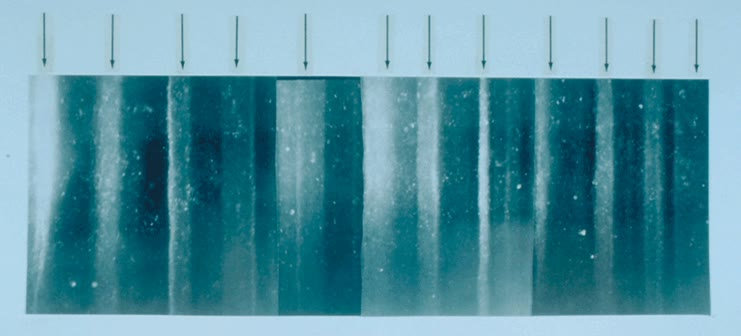
\includegraphics[width=0.72\linewidth]{images/book4/b2-24-gisp2-layers.jpg}
\par\smallskip{\small मध्य ग्रीनलैंड के GISP2 बर्फ़ के कोर का \qty{1855}{m}
गहराई से एक खंड, नीचे से प्रकाशित, ग्रीष्म और शीत ऋतु की बारी-बारी से आती परतों के साथ (तीर
मूल स्लाइड के हैं)। शुष्क उत्तरी ग्रीष्म के दौरान आर्कटिक कनाडा और तटीय ग्रीनलैंड की धूल
पवन द्वारा हिमचादर पर लाई जाती है।
(Anthony Gow, U.S.\ Army Corps of Engineers CRREL, NOAA Paleoclimatology slide set, सार्वजनिक डोमेन,
विकिमीडिया कॉमन्स के माध्यम से।)}
\end{omfigure}
% ledger: photo:b2-24-gisp2, noaa:gisp2-layers

\begin{inthelab}[बर्फ़ का कोर काटना]
\begin{minipage}[t]{0.54\linewidth}\vspace{0pt}
एक राष्ट्रीय बर्फ़-कोर सुविधा में कोर नलियों में रखे जाते हैं, प्रति नली एक मीटर कोर, एक
अभिलेखागार फ़्रीज़र में \qty{-36}{\celsius} पर; वैज्ञानिक एक परीक्षण कक्ष में
\qty{-24}{\celsius} पर काम करते हैं। जब कोई नया कोर आता है, तो एक कोर प्रसंस्करण पंक्ति बनती है: वैज्ञानिक और
कर्मचारी हर खंड को मापते हैं, सूचीबद्ध करते हैं और काटते हैं, सामान्यतः प्रतिदिन 30 से \qty{35}{m}, इसलिए
\qty{1000}{m} लंबे कोर में छह से आठ सप्ताह लगते हैं। एक शोधकर्ता रंदे से कोर को चिकना छीलता है
और उसकी विद्युत चालकता मापता है, जो परतों को परिभाषित करने और दिनांकित करने की एक कुंजी है; दूसरा
उन टुकड़ों को आरी से काटता है जिनकी फँसी हुई वायु का कार्बन डाइऑक्साइड और मीथेन के लिए विश्लेषण होगा; फिर नमूने
उन प्रयोगशालाओं को भेजे जाते हैं जो उन्हें मापती हैं। EPICA डोम~C पर $\delta$D
प्रोफ़ाइल का हर नमूना \qty{55}{cm} बर्फ़ था।
\end{minipage}\hfill
\begin{minipage}[t]{0.42\linewidth}\vspace{0pt}
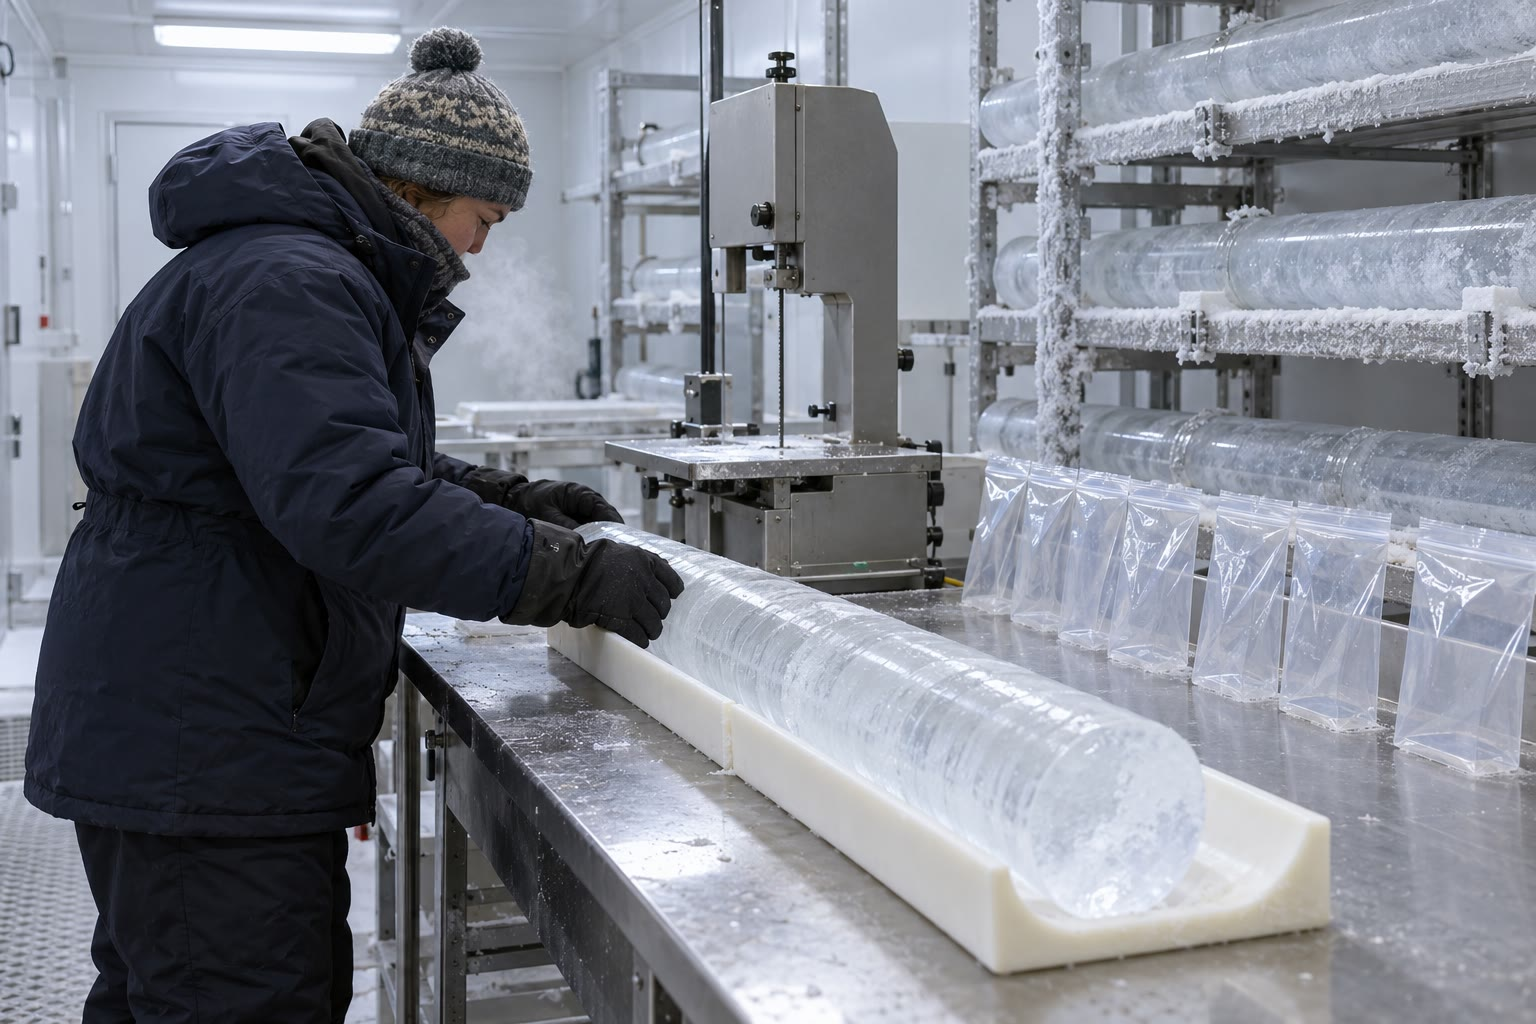
\includegraphics[width=\linewidth]{images/book4/ai/b2-24-cold-lab.jpg}

{\scriptsize एक शीत प्रयोगशाला की बेंच पर बर्फ़ के कोर का एक टुकड़ा, एक बैंड आरी और नमूना
थैलियों के पास (AI से बनाया गया चित्रण)।}
\end{minipage}
\end{inthelab}
% ledger: nsficf:cpl, jouzel07:edc-corr

\section{अन्य प्रॉक्सी, अन्य अभिलेखागार}\label{sec:b2:climate-proxies:others}

\subsection*{सीपियों का मैग्नीशियम}

फ़ोरामिनिफ़ेरा का कैल्साइट कैल्शियम के स्थान पर थोड़ा मैग्नीशियम ग्रहण करता है, और जल जितना गर्म हो
उतना अधिक। यह अनुपात जल के समस्थानिक संघटन पर निर्भर नहीं करता, इसलिए वह
वह तापमान देता है जिसकी $\delta^{18}$O समीकरण को आवश्यकता है।

\begin{definition}[Mg/Ca अनुपात (प्रॉक्सी)]\label{def:b2:climate-proxies:mgca}
\emph{Mg/Ca अनुपात (प्रॉक्सी)}\index{Mg/Ca अनुपात (प्रॉक्सी)} फ़ोरामिनिफ़ेरा की सीपियों के कैल्साइट में
मैग्नीशियम और कैल्शियम का अनुपात है, \unit{mmol/mol} में, जिसे एक घातांकी अंशांकन
के माध्यम से उस जल के तापमान के माप के रूप में प्रयुक्त किया जाता है जिसमें सीपी बढ़ी,
\[
  \text{Mg/Ca} = B\,\mathrm{e}^{A T},
\]
जहाँ प्लवकी जातियों के लिए $A$ \qty{0.09}{\per\celsius} के निकट है और $B$ जाति-विशिष्ट है।
\end{definition}
% ledger: groeneveld19:anand, morley24:mgca, miller20:paleotemp

$A = 0.09$ के साथ अनुपात प्रति अंश $\mathrm{e}^{0.09} - 1 = \qty{9.4}{\percent}$ बढ़ता है,
तापमान चाहे जो हो। ठंडे जलों की एक प्लवकी जाति के लिए, केवल तापमान से पूर्वानुमानित अंशांकन
$\text{Mg/Ca} = 0.4\,\mathrm{e}^{0.09T}$ है; प्लवक-जालों और उत्तर अटलांटिक कोरों के शीर्षों की 235 सीपियों पर
एक समंजन $0.372\,\mathrm{e}^{0.0936T}$ देता है, $r^2 = 0.90$ के साथ।
निम्न तापमानों पर मापे गए अनुपात वक्र से हट जाते हैं, और इस विचलन का श्रेय
समुद्री जल में कार्बोनेट आयन की सांद्रता को दिया जाता है: कोई प्रॉक्सी विरले ही केवल एक चर पर निर्भर करता है।
नितलवासी जातियाँ कम संवेदनशील हैं, अवसाद में रहने वाली निम्न-मैग्नीशियम जातियों के लिए
प्रति अंश लगभग \qty{0.1}{mmol/mol}।
% ledger: morley24:mgca, wharton26:deep

\begin{omfigure}
\centering
% figdata/bachelor-2/proxies.py part calib
\begin{tikzpicture}
\begin{groupplot}[group style={group size=2 by 1, horizontal sep=1.7cm},
  tick label style={font=\scriptsize}, label style={font=\small}, height=5.2cm,
  width=0.48\linewidth]
\nextgroupplot[xmin=-2, xmax=14, ymin=0, ymax=3.8, xlabel={$T$ (\unit{\celsius})},
  ylabel={$\delta^{18}\mathrm{O}_{\mathrm{b}} - \delta^{18}\mathrm{O}_{\mathrm{sw}}$ (प्रति मिल)},
  xtick={0,4,...,12}, title={क\enspace नितलवासी $\delta^{18}$O}, title style={font=\scriptsize}]
\addplot[black, thick] table[x=T, y=dd_benthic] {figdata/out/bachelor-2-proxies-calib.dat};
\nextgroupplot[xmin=0, xmax=30, ymin=0, ymax=6.5, xlabel={$T$ (\unit{\celsius})},
  ylabel={Mg/Ca (\unit{mmol/mol})}, xtick={0,5,...,30}, title={ख\enspace प्लवकी Mg/Ca},
  title style={font=\scriptsize},
  legend style={font=\scriptsize, at={(0.03,0.97)}, anchor=north west, draw=none},
  legend cell align=left]
\addplot[ocRed, thick] table[x=T, y=mgca_pred] {figdata/out/bachelor-2-proxies-calib.dat};
\addlegendentry{$0.4\,\mathrm{e}^{0.09T}$}
\addplot[ocBlue, thick, densely dashed] table[x=T, y=mgca_fit]
  {figdata/out/bachelor-2-proxies-calib.dat};
\addlegendentry{$0.372\,\mathrm{e}^{0.0936T}$}
\end{groupplot}
\end{tikzpicture}
\par\smallskip{\small दो अंशांकन। (क) \cref{prop:b2:climate-proxies:benthic} का
नितलवासी अंशांकन: ठंडा होने के हर अंश पर कैल्साइट जल से (अपने-अपने
पैमानों पर) \num{0.21} प्रति मिल और भारी होता है। (ख) एक प्लवकी
जाति का Mg/Ca, केवल तापमान से पूर्वानुमानित और 235 सीपियों पर समंजित।}
\end{omfigure}
% ledger: miller20:paleotemp, morley24:mgca

उन्हीं सीपियों पर मापे जाने पर, Mg/Ca और $\delta^{18}$O दो अज्ञातों के लिए दो समीकरण देते हैं: Mg/Ca
$T$ देता है, और फिर \cref{prop:b2:climate-proxies:benthic}
$\delta^{18}\mathrm{O}_{\mathrm{sw}}$, यानी हिम-आयतन संकेत, देता है। उत्तर-पश्चिम अटलांटिक के गहरे भाग की
नितलवासी सीपियों पर लागू करने पर, यह विधि अंतिम हिमनदीय अधिकतम के जल को आज के जल से केवल लगभग
\qty{2}{\celsius} ठंडा पाती है ($-1.78 \pm \qty{0.56}{\celsius}$), जबकि
छिद्र-जलों से प्राप्त अनुमान हिमनदीय महासागर में दोनों गहरी जल-राशियों को हिमांक के निकट, $-1.1$ और
\qty{-1.9}{\celsius} पर, रखते हैं, जहाँ आज वे 2 से \qty{4}{\celsius} और 0 से \qty{1}{\celsius} पर हैं।
% ledger: miller20:paleotemp, wharton26:deep

\subsection*{वृक्ष-वलय}

\begin{definition}[वृक्ष-वलय जलवायु-विज्ञान; परस्पर काल-मिलान]\label{def:b2:climate-proxies:dendro}
\emph{वृक्ष-वलय जलवायु-विज्ञान}\index{वृक्ष-वलय जलवायु-विज्ञान} वृक्षों के वार्षिक वृद्धि-वलयों से, यानी
उनकी चौड़ाई, उनकी लकड़ी के घनत्व और उनके समस्थानिक संघटन से, अतीत की जलवायु का
पुनर्निर्माण है। \emph{परस्पर काल-मिलान}\index{परस्पर काल-मिलान} वृक्षों के बीच चौड़े और
संकरे वलयों के प्रतिरूप का मिलान है, जो हर वलय को उसका निरपेक्ष कैलेंडर वर्ष देता है और उन
वलयों को प्रकट करता है जो किसी एक वृक्ष में स्थानीय रूप से अनुपस्थित हैं।
\end{definition}
% ledger: bebchuk26:crossdating, bebchuk26:absent-rings, ncei:tree-ring, ncei:proxy

अनुकूल परिस्थितियों में वलय अधिक चौड़ा होता है। \omterm{def:b2:climate-proxies:dendro}{परस्पर काल-मिलान} जलवायु की दृष्टि से चरम स्थलों पर विश्वसनीय है, जहाँ एक
जलवायु कारक सभी वृक्षों की वृद्धि को सीमित करता है, जिससे उनका प्रतिरूप एक जैसा होता है; वह वहाँ
विफल हो सकता है जहाँ कोई एक कारक प्रभावी नहीं होता, और जहाँ अनेक वलय स्थानीय रूप से अनुपस्थित होते हैं।
जीवित वृक्षों, पुरानी इमारती लकड़ियों और दबी हुई लकड़ी के प्रतिरूपों को एक-दूसरे पर चढ़ाकर कालक्रम को
वर्ष-दर-वर्ष पीछे बढ़ाया जाता है; एक हाल के अध्ययन ने पूर्वी इंग्लैंड के 100 उप-जीवाश्म यू वृक्षों के एक कालक्रम को
2668 से 2213 ईसा पूर्व तक के 456 वर्षों में दिनांकित किया, $\delta^{18}$O का उपयोग करके, जो उनके \num{1500} से अधिक वलयों पर
मापा गया और एक निरपेक्ष रूप से दिनांकित बांज कालक्रम से मिलाया गया। अंतरराष्ट्रीय वृक्ष-वलय डेटा बैंक छह महाद्वीपों के
\num{5000} से अधिक स्थलों की वलय-चौड़ाइयाँ, घनत्व, समस्थानिक और कालक्रम रखता है।
% ledger: ncei:proxy, bebchuk26:crossdating, bebchuk26:absent-rings, ncei:tree-ring

\subsection*{गुफाएँ और झीलें}

\begin{definition}[स्पेलियोथेम; वार्व]\label{def:b2:climate-proxies:archives}
\emph{स्पेलियोथेम}\index{स्पेलियोथेम} किसी गुफा के भीतर भूजल से बना एक खनिज
निक्षेप है: स्टैलेग्माइट, स्टैलेक्टाइट और अन्य रूप। \emph{वार्व}\index{वार्व}
किसी झील या समुद्र-तल के अवसाद में एक वर्ष का निक्षेप है, सामान्यतः विषम संघटन की
पटलिकाओं का एक जोड़ा, एक ग्रीष्म में और एक वर्ष के शेष भाग में बिछा हुआ।
\end{definition}
% ledger: ncei:speleothem, mccarthy23:varves

\omterm{def:b2:climate-proxies:archives}{स्पेलियोथेम} गुफा तक पहुँचने वाले भूजल से परत-दर-परत बढ़ते हैं; उनकी परतों की मोटाई
और उनके समस्थानिक अभिलेख अतीत की जलवायु परिस्थितियाँ बताते हैं। कुछ वार्षिक रूप से पट्टित होते हैं,
और कुछ में ऐसे यौगिक होते हैं जिनका रेडियोमितीय काल-निर्धारण किया जा सकता है। ग्रीनलैंड के कोरों का काल-मापक्रम
पिछले \num{60000} वर्षों में हुलु गुफा के \omterm{def:b2:climate-proxies:archives}{स्पेलियोथेमों} के काल-मापक्रम से 800 वर्षों के भीतर मेल खाता है: दो
अभिलेखागार, भिन्न विधियों से दिनांकित, एक-दूसरे की जाँच करते हैं।
% ledger: ncei:speleothem, svensson08:gicc05

\begin{omfigure}
\centering
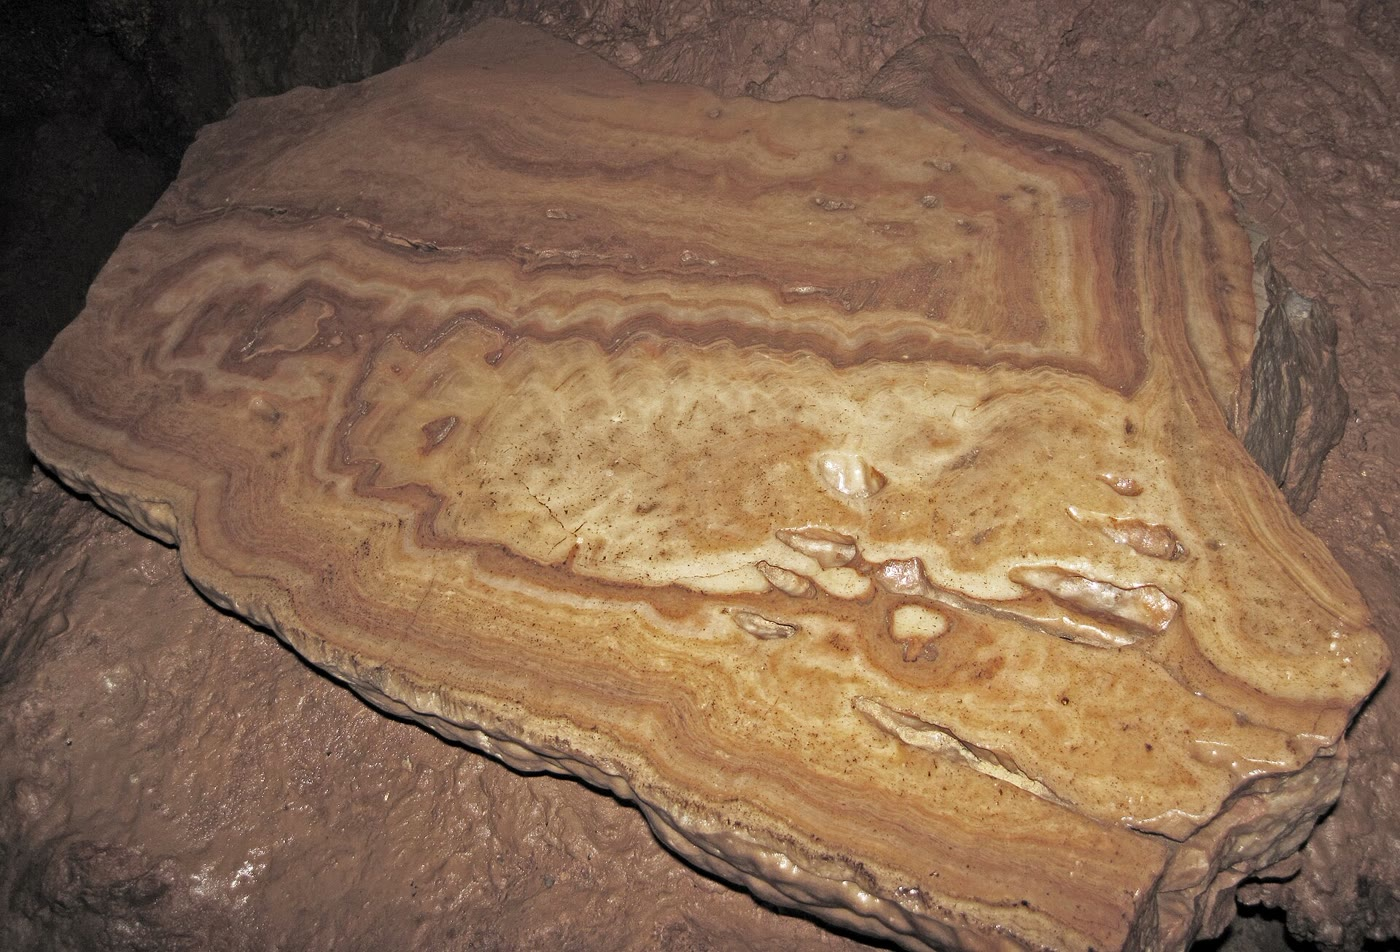
\includegraphics[width=0.62\linewidth]{images/book4/b2-24-speleothem.jpg}
\par\smallskip{\small केंटकी के डायमंड केवर्न्स से एक कैल्साइट \omterm{def:b2:climate-proxies:archives}{स्पेलियोथेम} का कटा और पॉलिश किया हुआ खंड,
लौह ऑक्साइड अशुद्धियों से रंगा हुआ: हर पट्टी कभी निक्षेप की सतह थी।
(James St.~John, CC BY 2.0, विकिमीडिया कॉमन्स के माध्यम से।)}
\end{omfigure}
% ledger: photo:b2-24-speleothem

ओंटारियो की क्रॉफ़र्ड झील की गहरी द्रोणी में तली का जल, जो अपने ऊपर के जल से अधिक लवणीय और अधिक क्षारीय है,
कीचड़ को हिलाने लायक बड़े कोई जंतु नहीं रखता, यद्यपि वह भली-भाँति
ऑक्सीजनित है, और हर वर्ष एक युग्म जोड़ता है: कार्बनिक पदार्थ की एक परत, जिसके ऊपर वह
कैल्साइट होता है जो हर ग्रीष्म क्षारीय सतही जल से अवक्षेपित होता है। झील के अवसाद आसपास की
वनस्पति के पराग भी रखते हैं, जिन्हें पराग-विश्लेषण द्वारा पढ़ा जाता है; वार्वित हों या नहीं, वे स्थल का
अभिलेख रखते हैं।
% ledger: mccarthy23:varves, mccarthy23:no-bioturbation, ncei:pollen

\section{आयु-मॉडल}\label{sec:b2:climate-proxies:age}

बिना तिथि का प्रॉक्सी एक कौतूहल-मात्र है। हर अभिलेखागार को गहराई, या वलय, या
पट्टी, और आयु के बीच एक संबंध चाहिए।

\begin{definition}[आयु-मॉडल; वार्षिक परत गणना]\label{def:b2:climate-proxies:age-model}
\emph{आयु-मॉडल}\index{आयु-मॉडल} वह फलन है जो किसी अभिलेखागार की हर गहराई को उसकी अनिश्चितता सहित
एक आयु देता है। \emph{वार्षिक परत गणना}\index{वार्षिक परत गणना} ऊपर से नीचे की ओर उन परतों को
गिनकर आयु-मॉडल बनाती है जिनमें से हर एक एक वर्ष दर्ज करती है (बर्फ़ की परतें, \omterm{def:b2:climate-proxies:archives}{वार्व},
पट्टियाँ), और जिस परत की वार्षिक प्रकृति संदिग्ध हो उसे आधा वर्ष, धन या ऋण
आधा वर्ष, गिना जाता है।
\end{definition}
% ledger: svensson08:gicc05, mccarthy23:varves

\begin{method}[आयु-मॉडल बनाना]\label{met:b2:climate-proxies:age-model}
\begin{enumerate}
  \item जहाँ अभिलेखागार में वार्षिक परतें हों, उन्हें किसी ज्ञात शीर्ष से गिनिए, और अनिश्चित परतों को
        अलग से दर्ज कीजिए।
  \item जहाँ वे न हों, या उनका विभेदन न हो सके, \emph{बंधन बिंदु} स्थिर कीजिए: ऐसी गहराइयाँ जो
        स्वतंत्र रूप से दिनांकित हों, रेडियोकार्बन या अन्य रेडियोमितीय विधियों से, किसी दिनांकित ज्वालामुखीय राख से, या
        किसी भली-भाँति दिनांकित अभिलेख से मिलान करके।
  \item बंधन बिंदुओं के बीच अंतर्वेशन कीजिए, गहराई में रैखिक रूप से यदि इससे बेहतर कुछ ज्ञात न हो, या
        इस मॉडल के साथ कि अभिलेखागार कैसे संचित हुआ और पतला हुआ।
  \item हर चरण की अनिश्चितता को हर गहराई तक ले जाइए।
\end{enumerate}
\end{method}
% ledger: svensson08:gicc05, noaa:gisp2-layers, ncei:speleothem

ग्रीनलैंड बर्फ़-कोर कालक्रम 2005, GICC05, पिछले \num{60000} वर्षों में तीन ग्रीनलैंड कोरों में वार्षिक परतें गिनता है, और
हिमनदीय भाग में केवल नॉर्थग्रिप कोर में; उसकी आयुएँ
ईसवी सन् 2000 से पहले के वर्षों में दी जाती हैं, जिन्हें b2k लिखा जाता है। अनिश्चित परतें, जो $\frac12 \pm \frac12$ गिनी जाती हैं,
जुड़कर \emph{अधिकतम गणना-त्रुटि} बनाती हैं, जिसे लेखक दो मानक विचलन मानते हैं।
होलोसीन के आरंभ पर, 11\,703 वर्ष b2k, वह 50 वर्ष है; ग्रीनलैंड
इंटरस्टेडियल 17 के आरंभ पर, \num{59440} वर्ष b2k, वह \num{1287} वर्ष है।
% ledger: svensson08:gicc05, svensson08:table1

\begin{proposition}[गणना-त्रुटि की वृद्धि]\label{prop:b2:climate-proxies:counting}
मान लीजिए किसी गणना में $n$ अनिश्चित परतें हैं, हर एक $\frac12$ गिनी गई, मानक
विचलन $\frac12$ की त्रुटि के साथ। यदि परतों की त्रुटियाँ स्वतंत्र हैं, तो कुल का मानक विचलन
$\frac12\sqrt{n}$ है; यदि वे सब एक ही चिह्न की हैं, तो कुल की त्रुटि
$\frac12 n$ है।
\end{proposition}

\begin{proof}
स्वतंत्र त्रुटियों के योग का प्रसरण उनके प्रसरणों का योग है: $n \times
(\frac12)^2$, जिसका वर्गमूल $\frac12\sqrt{n}$ है। यदि हर परत एक ही दिशा में त्रुटि करती है, तो
त्रुटियाँ संख्याओं की तरह जुड़ती हैं: $n \times \frac12$।
\end{proof}

GI-17 पर अधिकतम गणना-त्रुटि के \num{1287} वर्षों का अर्थ है \num{2574} अनिश्चित परतें। यदि
उनकी त्रुटियाँ स्वतंत्र होतीं, तो कुल केवल $\frac12\sqrt{2574} = 25$ वर्षों से अनिश्चित होता।
रैखिक योग सतर्क विकल्प है: बर्फ़ के एक खंड की संदिग्ध परतों को वही गणक उन्हीं
मानदंडों से आँकते हैं, और उनकी त्रुटियों के एक-दूसरे को निरस्त करने की अपेक्षा का कोई कारण नहीं है।
अभिलेख के पुराने भाग को दो लेखकों ने स्वतंत्र रूप से गिना; उनकी गणनाएँ
निरपेक्ष त्रुटि से कम भिन्न हैं, यद्यपि स्थानीय रूप से अंतिम गणना-त्रुटि से अधिक। अधिकतम
गणना-त्रुटि होलोसीन में किसी खंड द्वारा आच्छादित समय का औसतन लगभग \qty{1}{\percent} है और
हिमनदीय भाग में \qty{5}{\percent}।
% ledger: svensson08:gicc05, svensson08:table1, svensson08:two-counters

\begin{omfigure}
\centering
% figdata/bachelor-2/proxies.py part gicc05
\begin{tikzpicture}
\begin{groupplot}[group style={group size=2 by 1, horizontal sep=1.7cm},
  tick label style={font=\scriptsize}, label style={font=\small}, height=5.4cm,
  width=0.48\linewidth, xmin=0, xmax=62, xlabel={GICC05 आयु (\unit{ka} b2k)}]
\nextgroupplot[ymin=1450, ymax=2450, y dir=reverse, ylabel={नॉर्थग्रिप गहराई (\unit{m})},
  title={क\enspace गहराई और आयु}, title style={font=\scriptsize}]
\addplot[black, mark=*, mark size=1.1pt] table[x=age_ka, y=depth_m]
  {figdata/out/bachelor-2-proxies-gicc05.dat};
\nextgroupplot[ymode=log, ymin=2, ymax=30000, ylabel={अनिश्चितता (वर्ष)},
  title={ख\enspace गणना-अनिश्चितता}, title style={font=\scriptsize},
  legend style={font=\scriptsize, at={(0.03,0.97)}, anchor=north west, draw=none},
  legend cell align=left]
\addplot[ocRed, mark=*, mark size=1.1pt] table[x=age_ka, y=err_yr]
  {figdata/out/bachelor-2-proxies-gicc05.dat};
\addlegendentry{अधिकतम गणना-त्रुटि}
\addplot[ocBlue, mark=o, mark size=1.1pt] table[x=age_ka, y=err_random_yr]
  {figdata/out/bachelor-2-proxies-gicc05.dat};
\addlegendentry{यदि स्वतंत्र}
\end{groupplot}
\end{tikzpicture}
\par\smallskip{\small होलोसीन के आरंभ से \qty{59.44}{ka} तक 18 जलवायु घटनाओं पर GICC05
कालक्रम: (क) नॉर्थग्रिप कोर में आयु के सापेक्ष गहराई; वक्र चपटा होता जाता है क्योंकि वार्षिक
परतें गहराई के साथ पतली होती हैं, हर हज़ार वर्ष बर्फ़ के कम मीटर घेरते हैं; (ख) अधिकतम गणना-त्रुटि, और वह त्रुटि जो उतनी ही अनिश्चित
परतें देतीं यदि उनकी त्रुटियाँ स्वतंत्र होतीं (\cref{prop:b2:climate-proxies:counting});
लघुगणकीय पैमाना। डेटा: Svensson और अन्य (2008), तालिका 1।}
\end{omfigure}
% ledger: svensson08:table1, svensson08:gicc05

वार्षिक परतें गहराई के साथ पतली होती हैं, क्योंकि बर्फ़ डूबते हुए बहती और फैलती है: होलोसीन के आरंभ
और GI-1 के बीच नॉर्थग्रिप में माध्य परत \qty{3.75}{cm} मोटी है; GI-16 और
GI-17 के बीच \qty{1.54}{cm}; लगभग \qty{100}{ka} पर प्रवाह मॉडल उसे \qty{1}{cm} के निकट रखते हैं। परतें जितनी पतली, उन्हें
अलग पहचानना उतना ही कठिन।
% ledger: svensson08:table1, svensson08:gicc05

\section{अंशांकन}\label{sec:b2:climate-proxies:calibration}

किसी प्रॉक्सी से पढ़ी गई हर संख्या एक अंशांकन से होकर आती है।

\begin{definition}[प्रॉक्सी अंशांकन]\label{def:b2:climate-proxies:calibration}
\emph{प्रॉक्सी अंशांकन}\index{प्रॉक्सी अंशांकन} वह आनुभविक या सैद्धांतिक संबंध है जो
किसी प्रॉक्सी के मान को उस जलवायु चर में बदलता है जिसका वह स्थान लेता है, ऐसे नमूनों पर स्थापित जिनके
लिए दोनों ज्ञात हैं, साथ में उसकी अनिश्चितता और परिस्थितियों का वह परास जिस पर वह
वैध है।
\end{definition}
% ledger: morley24:mgca, miller20:paleotemp

जिन नमूनों के लिए दोनों ज्ञात हैं वे आधुनिक हैं: प्लवक-जालों में पकड़ी गई सीपियाँ, ऊपर के जल से तुलना किए गए अवसाद-कोरों के शीर्ष, अपने स्थल के तापमान से तुलना की गई
हाल की हिम, किसी मौसम-वेधशाला के अभिलेखों से तुलना किए गए वृक्षों के बाहरी वलय।
फिर संबंध को न्यूनतम वर्गों से समंजित किया जाता है; Mg/Ca अंशांकन जैसे घातांकी नियम के लिए
समंजन लघुगणक पर किया जाता है, जो $\text{Mg/Ca} = B\,\mathrm{e}^{AT}$ को
सरल रेखा $\ln(\text{Mg/Ca}) = \ln B + AT$ में बदल देता है। किसी अंशांकन का सत्यापन उन नमूनों पर होता है जो
उसके समंजन में प्रयुक्त नहीं हुए: आधुनिक आँकड़ों का एक भाग अलग रखा जाता है और उसका पूर्वानुमान किया जाता है।
% ledger: morley24:mgca, werner18:slopes, ncei:tree-ring

तीन सीमाएँ बची रहती हैं। स्थान के आर-पार, आज एक जगह से दूसरी जगह, मापा गया अंशांकन समय में
लागू न भी हो, जैसा ग्रीनलैंड की बर्फ़ ने दिखाया है। आज की परिस्थितियों के परास पर मापे गए अंशांकन का
बहिर्वेशन सावधानी से करना चाहिए: सीपियों का Mg/Ca निम्न तापमानों पर अपने नियम से हट जाता है, जहाँ
एक अन्य चर, कार्बोनेट आयन, हावी हो जाता है। और जो संबंध छोटे परास पर रैखिक है वह
बड़े परास पर रैखिक न भी हो, जैसे \omterm{def:b2:climate-proxies:ice-volume}{हिम-आयतन प्रभाव} नहीं है। इस अध्याय की विधि
इन सबका उत्तर एक ही तरह देती है: एक ही नमूने पर दो स्वतंत्र प्रॉक्सी मापिए, और हर एक को
दूसरे की जाँच करने दीजिए।
% ledger: werner18:slopes, morley24:mgca, rohling21:linear

\section*{अभ्यास}\label{sec:b2:climate-proxies:exercises}

अभ्यासों के आँकड़े, अन्यथा न कहा जाए तो: माध्य महासागर गहराई $H = \qty{3682.2}{m}$, महासागर का
क्षेत्रफल \qty{361.84e6}{km^2}; \cref{prop:b2:climate-proxies:benthic} का नितलवासी अंशांकन;
प्लवकी अंशांकन $\text{Mg/Ca} = 0.4\,\mathrm{e}^{0.09T}$ (\unit{mmol/mol}, \unit{\celsius});
जलों और बर्फ़ के $\delta$ मान प्रति मिल \omterm{def:b2:isotope-geochemistry:standards}{VSMOW} में, कैल्साइट के प्रति मिल \omterm{def:b2:isotope-geochemistry:standards}{VPDB} में।
% ledger: charette:ocean-volume, miller20:paleotemp, morley24:mgca

\begin{exercise}[$\star$]\label{exo:b2:climate-proxies:1}
आज महाद्वीपीय बर्फ़ लगभग \qty{27.5e6}{km^3} और महासागर \qty{1350e6}{km^3} जल
रखता है (आयतनों को जल की मात्राएँ मानिए)। (क)~यदि बर्फ़ का माध्य $\delta^{18}$O $-30$ प्रति
मिल और महासागर का 0 है, तो मीठे जल की उपेक्षा करते हुए पूरे जलमंडल का $\delta^{18}$O क्या है?
(ख)~यदि सारी बर्फ़ पिघल जाए, तो महासागर का $\delta^{18}$O क्या हो जाएगा? (ग)~जल का कितना
अंश बर्फ़ है?
\end{exercise}
% ledger: white13c9:ice-mass

\begin{exercise}[$\star$]\label{exo:b2:climate-proxies:2}
एक नितलवासी सीपी का $\delta^{18}\mathrm{O}_{\mathrm{b}} = 2.50$ प्रति मिल है। (क)~उसका
तापमान परिकलित कीजिए यदि समुद्री जल का $\delta^{18}\mathrm{O}_{\mathrm{sw}} = 0$ था। (ख)~उसे परिकलित कीजिए यदि
समुद्री जल का $+1.0$ प्रति मिल था। (ग)~उसी $0$ प्रति मिल वाले जल की एक दूसरी सीपी का
$2.71$ प्रति मिल है: उसका जल कितना अधिक ठंडा था?
\end{exercise}
% ledger: miller20:paleotemp

\begin{exercise}[$\star$]\label{exo:b2:climate-proxies:3}
(क)~\qty{10}{\celsius} और
\qty{20}{\celsius} पर प्लवकी अंशांकन का Mg/Ca अनुपात परिकलित कीजिए। (ख)~इन दस अंशों में अनुपात किस गुणक से बढ़ता है, और प्रति अंश
कितने प्रतिशत? (ग)~Mg/Ca = 2.0 और
\qty{1.0}{mmol/mol} वाली सीपियों का तापमान परिकलित कीजिए।
\end{exercise}
% ledger: morley24:mgca

\begin{exercise}[$\star$]\label{exo:b2:climate-proxies:4}
उप-जीवाश्म यू वृक्षों का एक कालक्रम 2668 से 2213 ईसा पूर्व तक चलता है। (क)~दोनों अंतिम वर्षों को गिनते हुए,
वह कितने वर्षों को आच्छादित करता है? (ख)~अनेक वृक्षों से बना कालक्रम किसी एक वृक्ष के वलयों की गिनती से
अधिक भरोसे के योग्य क्यों है? (ग)~आप ठंडी वृक्ष-रेखा के पास के वृक्षों के लिए \omterm{def:b2:climate-proxies:dendro}{परस्पर काल-मिलान} को किसी सौम्य, नम
निचले वन के वृक्षों की तुलना में आसान होने की अपेक्षा क्यों करेंगे?
\end{exercise}
% ledger: bebchuk26:crossdating

\begin{exercise}[$\star\star$]\label{exo:b2:climate-proxies:5}
(क)~\cref{prop:b2:climate-proxies:mass-balance} से \qty{125}{m} और \qty{134}{m} के समुद्र-तल
पतन के लिए, $-40$ प्रति मिल की बर्फ़ के साथ, \omterm{def:b2:climate-proxies:ice-volume}{हिम-आयतन प्रभाव} परिकलित कीजिए। (ख)~उसे
\qty{130}{m} के लिए $-30$, $-35$ और $-50$ प्रति मिल की बर्फ़ के साथ परिकलित कीजिए। (ग)~बर्फ़ का कौन-सा माध्य संघटन
\qty{130}{m} के पतन के प्रभाव को छिद्र-जलों में मापे गए \num{1.0} प्रति मिल के बराबर
बना देगा? वर्तमान हिमचादरों के संघटनों से तुलना कीजिए।
\end{exercise}
% ledger: ipcc:lgm-sea, white:d18o, miller20:ice-cal, wharton26:deep

\begin{exercise}[$\star\star$]\label{exo:b2:climate-proxies:6}
एक ही प्लवकी जाति के Mg/Ca के दो अंशांकनों की तुलना कीजिए: केवल
तापमान से पूर्वानुमानित, $0.4\,\mathrm{e}^{0.09T}$, और समंजन $0.372\,\mathrm{e}^{0.0936T}$। (क)~किस
तापमान पर वे सहमत होते हैं? (ख)~\qty{2}{\celsius} पर समंजित अनुपात पूर्वानुमानित अनुपात से कितने प्रतिशत
कम है? (ग)~\qty{2}{\celsius} पर बढ़ी एक सीपी समंजित नियम का पालन करती है; पूर्वानुमानित नियम उसके लिए कौन-सा
तापमान देगा?
\end{exercise}
% ledger: morley24:mgca

\begin{exercise}[$\star\star$]\label{exo:b2:climate-proxies:7}
नॉर्थग्रिप कोर में होलोसीन का आरंभ \qty{1492.45}{m} और \num{11703} वर्ष
b2k पर है, GI-1 का आरंभ \qty{1604.64}{m} और \num{14692} वर्ष पर; GI-16 का आरंभ
\qty{2402.55}{m} और \num{58280} वर्ष पर, GI-17 का \qty{2420.44}{m} और \num{59440} वर्ष पर।
(क)~हर अंतराल में वार्षिक परतों की माध्य मोटाई परिकलित कीजिए। (ख)~वे अधिक गहराई पर पतली
क्यों हैं? (ग)~किसी गहराई पर \omterm{def:b2:climate-proxies:age-model}{वार्षिक परत गणना} असंभव क्यों हो जाती है?
\end{exercise}
% ledger: svensson08:table1, svensson08:gicc05

\begin{exercise}[$\star\star$]\label{exo:b2:climate-proxies:8}
\cref{exo:b2:climate-proxies:7} के पहले दो बंधन बिंदुओं का उपयोग कीजिए, 50
और 93 वर्षों की अधिकतम गणना-त्रुटियों के साथ। (क)~गहराई में रैखिक अंतर्वेशन से \qty{1550}{m} पर बर्फ़ की आयु दीजिए।
(ख)~उसे 1950 से पहले के वर्षों में व्यक्त कीजिए। (ग)~अनिश्चितता का उसी प्रकार अंतर्वेशन कीजिए।
\end{exercise}
% ledger: svensson08:table1

\begin{exercise}[$\star\star$]\label{exo:b2:climate-proxies:9}
GICC05 की अधिकतम गणना-त्रुटि GI-1 पर 93 वर्ष और GI-17 पर \num{1287} वर्ष है। (क)~हर एक कितनी
अनिश्चित परतों को निरूपित करती है? (ख)~यदि इन परतों की त्रुटियाँ स्वतंत्र होतीं, हर एक का मानक विचलन
आधा वर्ष, तो अनिश्चितता क्या होती? (ग)~हर स्थिति में रैखिक योग स्वतंत्र अनुमान से किस गुणक से
अधिक है, और यह गुणक गहराई के साथ क्यों बढ़ता है?
\end{exercise}
% ledger: svensson08:gicc05, svensson08:table1

\begin{exercise}[$\star\star\star$]\label{exo:b2:climate-proxies:10}
EPICA डोम~C पर बर्फ़ का माध्य $\delta$D पिछले दो हज़ार वर्षों में $-396.6$ प्रति मिल है
और $-441.7$ प्रति मिल, 19 से \qty{23}{ka} में। (क)~$\delta^{18}$O की अंटार्कटिक स्थानिक प्रवणता
\num{0.8} प्रति मिल प्रति अंश है। \omterm{prop:b2:isotope-geochemistry:mwl}{उल्कीय जल रेखा} से उसे $\delta$D की प्रवणता में बदलिए और
हिमनदीय शीतलन का आकलन कीजिए। (ख)~हिमनदीय महासागर \num{1.0} प्रति मिल भारी था,
$\delta^{18}$O में, इसलिए उससे बनी हिम भी भारी थी। यह मानते हुए कि महासागर का $\delta$D
आठ गुना बदला, हिमनदीय $\delta$D का सुधार कीजिए और शीतलन का फिर से आकलन कीजिए।
(ग)~दोनों अवधियों के लिए प्रकाशित विसंगति $-0.09$ और \qty{-9.39}{\celsius} है; इससे प्रति अंश $\delta$D की
कौन-सी प्रवणता निहित है, और प्रकाशित श्रेणी में कौन-सा अन्य सुधार शामिल है?
\end{exercise}
% ledger: data:b4-proxies, werner18:slopes, kc98:mwl, wharton26:deep, jouzel07:edc-corr

\begin{exercise}[$\star\star\star$]\label{exo:b2:climate-proxies:11}
किसी प्लवकी जाति के Mg/Ca का एक अंशांकन छह कोर-शीर्ष नमूनों का उपयोग करता है (जल का तापमान,
Mg/Ca \unit{mmol/mol} में): (4, 0.59), (8, 0.80), (12, 1.21), (16, 1.65), (20, 2.47), (24, 3.41)।
(क)~न्यूनतम वर्गों से $\ln(\text{Mg/Ca}) = \ln B + AT$ समंजित कीजिए, और $A$ और $B$ दीजिए। (ख)~लघुगणक के
अवशेष परिकलित कीजिए, और समंजन की तुलना नियम $0.4\,\mathrm{e}^{0.09T}$ से कीजिए। (ग)~Mg/Ca = 1.30 वाली
एक हिमनदीय सीपी का तापमान दीजिए। (घ)~एक सीपी का Mg/Ca = 0.45 है: उसका
तापमान परिकलित कीजिए, और बताइए कि यह मान पिछले मान से कम भरोसे के योग्य क्यों है।
\end{exercise}
% ledger: morley24:mgca

\begin{exercise}[$\star\star\star$]\label{exo:b2:climate-proxies:12}
एक हिमचादर दो चरणों में बढ़ती है: पहले समुद्र-तल के \qty{60}{m} को $-30$ प्रति मिल की बर्फ़ के रूप में संचित किया जाता है,
फिर \qty{70}{m} और $-45$ प्रति मिल की बर्फ़ के रूप में। (क)~दिखाइए कि बर्फ़ के अनेक भंडारों के लिए
\cref{prop:b2:climate-proxies:mass-balance} का द्रव्यमान संतुलन $(H - h)\,\Delta\delta = -\sum_i h_i\delta_i$
हो जाता है, और हर चरण के बाद \omterm{def:b2:climate-proxies:ice-volume}{हिम-आयतन प्रभाव} परिकलित कीजिए। (ख)~अंत में बर्फ़ का माध्य
संघटन क्या है? (ग)~अंतिम अवस्था पर अंशांकित एक रैखिक नियम
$\Delta\delta$ को समुद्र-तल में बदलता है। वह पहले चरण के लिए कितना समुद्र-तल पतन निकालेगा, और वह
क्यों चूकता है?
\end{exercise}
% ledger: rohling21:linear, white:d18o, miller20:ice-cal

\begin{problem}[{सप्ताहांत समस्या --- एक सीपी, दो संकेत}]\label{pb:b2:climate-proxies:1}
अंतिम हिमनदीय अधिकतम पर गहरा महासागर कितना अधिक ठंडा था? नितलवासी सीपियों का $\delta^{18}$O
उत्तर को बर्फ़ के आयतन के साथ मिला देता है; यह समस्या दोनों को अलग करती है।
अभ्यासों के आँकड़ों का उपयोग कीजिए; समुद्र-तल आज के तल से 125 से \qty{134}{m} नीचे था, और उत्तर अमेरिकी हिमचादर की
बर्फ़ का $\delta^{18}$O लगभग $-40$ प्रति मिल माना जाता है।

\medskip\noindent\textbf{भाग I --- स्थल पर बर्फ़।}
\begin{enumerate}
  \item \qty{130}{m} के समुद्र-तल पतन द्वारा महासागर से हटाए गए जल का आयतन परिकलित कीजिए।
  \item $-40$ प्रति मिल की बर्फ़ के साथ उस पतन का \omterm{def:b2:climate-proxies:ice-volume}{हिम-आयतन प्रभाव} परिकलित कीजिए।
  \item उसे \qty{125}{m} और \qty{134}{m} के पतनों के लिए परिकलित कीजिए।
  \item उसे \qty{130}{m} के लिए $-35$ और $-50$ प्रति मिल की बर्फ़ के साथ परिकलित कीजिए। कौन-सी अनिश्चितता
        अधिक मायने रखती है, समुद्र-तल की या बर्फ़ की?
  \item हिमनदीय अवसादों के छिद्र-जल $1.0 \pm 0.1$ प्रति मिल देते हैं। \qty{130}{m} के पतन को
        इसे उत्पन्न करने के लिए बर्फ़ के किस माध्य संघटन की आवश्यकता होगी?
  \item $-40$ प्रति मिल की बर्फ़ के साथ छोटे पतनों के लिए समुद्र-तल के प्रति मीटर विचलन परिकलित कीजिए, और
        दिनांकित समुद्र-तलों से व्युत्पन्न \num{0.011} प्रति मिल प्रति मीटर के मान से तुलना कीजिए।
\end{enumerate}

\medskip\noindent\textbf{भाग II --- दो थर्मामीटर।}
\begin{enumerate}[resume]
  \item \cref{prop:b2:climate-proxies:benthic} से दिखाइए कि स्थिर जल-संघटन पर \qty{1}{\celsius} की
        शीतलता $\delta^{18}\mathrm{O}_{\mathrm{b}}$ को \num{0.21} प्रति मिल बढ़ाती है।
  \item उस नितलवासी सीपी का $\delta^{18}\mathrm{O}_{\mathrm{b}}$ परिकलित कीजिए जो आज
        \qty{2.0}{\celsius} पर $\delta^{18}\mathrm{O}_{\mathrm{sw}} = 0$ वाले जल में बढ़ी।
  \item \qty{-1.0}{\celsius} पर
        $\delta^{18}\mathrm{O}_{\mathrm{sw}} = +1.0$ प्रति मिल वाले जल में बढ़ी एक हिमनदीय सीपी के लिए उसे परिकलित कीजिए। दोनों
        सीपियों के बीच परिवर्तन कितना है, और उसका कितना भाग जल के संघटन के कारण है?
  \item एक प्लवकी सीपी का Mg/Ca = \qty{2.0}{mmol/mol} है। उसका तापमान परिकलित कीजिए।
  \item निम्न-मैग्नीशियम नितलवासी सीपियाँ प्रति अंश लगभग \qty{0.1}{mmol/mol} बढ़ती हैं। एक हिमनदीय सीपी का
        Mg/Ca उसी स्थान की उसी जाति की एक आधुनिक सीपी से \qty{0.18}{mmol/mol} कम
        है। यह कितना शीतलन दर्शाता है?
  \item Mg/Ca ऐसा तापमान क्यों देता है जो बर्फ़ के आयतन पर निर्भर नहीं करता?
\end{enumerate}

\medskip\noindent\textbf{भाग III --- अवशेष।}
LR04 स्टैक आज \num{3.23} प्रति मिल पढ़ता है और \num{4.92} प्रति मिल औसतन, 19 से
\qty{23}{ka} में।
\begin{enumerate}[resume]
  \item आज और अंतिम हिमनदीय अधिकतम के बीच स्टैक का परिवर्तन परिकलित कीजिए।
  \item यदि वह सब \omterm{def:b2:climate-proxies:ice-volume}{हिम-आयतन प्रभाव} होता, $-40$ प्रति मिल की बर्फ़ के साथ, तो वह कितना समुद्र-तल पतन
        निहित करता (\cref{prop:b2:climate-proxies:mass-balance} को उलटिए)? क्या यह
        समुद्र-तल के साक्ष्य से संगत है?
  \item प्रश्न 2 का \omterm{def:b2:climate-proxies:ice-volume}{हिम-आयतन प्रभाव} लीजिए। तापमान के लिए कितना अवशेष बचता है, और
        वह गहरे जल का कितना शीतलन देता है?
  \item इसके बजाय छिद्र-जल का मान, \num{1.0} प्रति मिल, लीजिए। कितना अवशेष और कितना शीतलन?
  \item एक अन्य पुनर्निर्माण \num{0.25} प्रति मिल प्रति अंश का उपयोग करता है। उसके साथ दोनों आकलन दोहराइए।
  \item आज उत्तर अटलांटिक गहरा जल 2 से \qty{4}{\celsius} पर है और अंटार्कटिक तली
        जल 0 से \qty{1}{\celsius} पर; छिद्र-जल हिमनदीय महासागर में उन्हें $-1.1$ और \qty{-1.9}{\celsius}
        पर रखते हैं, और नितलवासी सीपियों का Mg/Ca उत्तर-पश्चिम अटलांटिक के गहरे भाग को
        केवल लगभग \qty{1.8}{\celsius} ठंडा पाता है। ये शीतलन का कौन-सा परास देते हैं, और प्रश्न 15 और 16 के
        दोनों आकलनों में से किसका समर्थन करते हैं?
\end{enumerate}

\medskip\noindent\textbf{भाग IV --- बर्फ़ से दृश्य।}
EPICA डोम~C पर माध्य $\delta$D पिछले दो हज़ार वर्षों में $-396.6$ प्रति मिल है और
$-441.7$ प्रति मिल, 19 से \qty{23}{ka} में; प्रकाशित तापमान विसंगति $-0.09$ और
\qty{-9.39}{\celsius} है।
\begin{enumerate}[resume]
  \item $\delta$D का परिवर्तन परिकलित कीजिए।
  \item $\delta^{18}$O की \num{0.8} प्रति मिल प्रति अंश की प्रवणता और \omterm{prop:b2:isotope-geochemistry:mwl}{उल्कीय जल रेखा} से,
        डोम~C पर शीतलन का आकलन कीजिए।
  \item प्रकाशित शीतलन परिकलित कीजिए, और प्रति अंश $\delta$D की वह प्रवणता जो वह निहित करता है।
  \item अंतिम हिमनदीय अधिकतम पर वैश्विक माध्य सतह 5 से \qty{7}{\celsius} ठंडी थी।
        डोम~C, पृथ्वी और गहरे महासागर के शीतलनों को क्रम में रखिए।
  \item गहरा महासागर अंटार्कटिका की सतह जितना ठंडा क्यों नहीं हो सकता था?
  \item सारांश में: हिम-आयतन के छिद्र-जल सुधार के साथ, अंतिम हिमनदीय अधिकतम पर गहरा महासागर
        आज की तुलना में कितना अधिक ठंडा था?
\end{enumerate}
\end{problem}
% ledger: charette:ocean-volume, ipcc:lgm-sea, miller20:ice-cal, white:d18o, white13c9:ice-volume, wharton26:deep, miller20:paleotemp, morley24:mgca, data:b4-proxies, rohling21:linear, werner18:slopes, kc98:mwl, ipcc:lgm-cooling
